\documentclass[DM,STP,toc]{lsstdoc}
\usepackage{pgfgantt}


%set the WP number or product here for the requirements
\def\product{Data Management}
\def\cycle{S17}

\setDocCompact{true}

%Product name first in title
\title    [Test Plan]  { \product ~Test Plan}

\author   {William O'Mullane, John Swinbank, Mario Juric, Frossie Economou}                % the author(s)
\setDocRef      {LDM-503} % the reference code
\setDocDate     {\today}              % the date of the issue
\setDocUpstreamLocation{\url{https://github.com/lsst/LDM-503}}
%
% a short abstract
%
\setDocAbstract {
This is the  Test Plan for \product. In it we define terms associated with testing and further test specifications for specific items.}

%
%
\setDocChangeRecord{%
	\addtohist{}{2017-01-13}{First draft}{William O'Mullane}
	\addtohist{1.0}{2017-06-30}{First approved release.}{William O'Mullane}
	\addtohist{1.1}{2017-07-04}{Minor cleanups for review. Approved in \href{https://jira.lsstcorp.org/browse/RFC-358}{RFC-358}.}{W.~O'Mullane}
	\addtohist{1.2}{2017-07-19}{Milestone alignment with plan }{W.~O'Mullane}
	\addtohist{}{\today}{Milestone alignment with PMCS and derived from it }{J.~Swinbank}
}


\begin{document}
%
% the title page
%
\maketitle



\section{Introduction \label{sect:intro}}

This document provides an introduction to and overview of the approach to verification and validation which bas been adopted by the LSST \product{} Subsystem.
Broadly, this approach consists of three aspects:

\begin{itemize}

  \item{\emph{Verification} that the \product{} system as delivered meets the requirements placed upon it;}
  \item{\emph{Validation} that the system as delivered meets the needs of the scientific community;}
  \item{\emph{Rehearsing} the sustained operation of the system in operational scenarios.}

\end{itemize}

This documentation describes how LSST \product{} is addressing each of these three requirements, and describes a series of high-level milestones and the accompanying test schedule.
In addition, it briefly discusses the software development infrastructure that has been developed to support all three of these aspects of testing.

\subsection{Objectives \label{sect:objectives}}

We describe the test and verification approach for \product{} and describe various constraints and limitations in the testing to be performed.
We also describe the program of rehearsals which will be undertaken to demonstrate the sustained operation of the \product{} system, and the validation exercises which will be performed on the partially and fully integrated system.
We do not describe all tests in detail; those are described in dedicated test specifications for major components of \product{}.

\subsection{Scope \label{sect:scope}}

This provides the approach and plan for all of \product{}.
It covers interfaces between \product{} and components from other LSST subsystems but nothing outside of \product{}.
This document is change-controlled by the DMCCB and will be updated in response to any requirements updates or changes of approach.

\subsection{Assumptions}

We will run large scale verification exercises in order to demonstrate the system's end-to-end capability against its design specifications.
A large amount of informal science verification and validation will be done in the the teams and documented in technical notes; in this test plan we are looking for verification of the broader system, demonstration of its \emph{operability} --- i.e. whether it can be run every day for the 10 year planned survey with a reasonable level of operational support --  and to validate its capability to meet the scientific expectations of the community.

\subsection{Applicable Documents \label{sect:ad}}

When applicable documents change a change may be required in this document.
\begin{tabbing}
AUTH-NUM\= \kill
\citeds{LPM-55} \>	LSST Quality  Assurance Plan \\
\citeds{LDM-148} \>	DM Architecture\\
\citeds{LDM-294} \>	DM Project Management Plan   \\
\citeds{LDM-639} \>	DM Acceptance Test Specification \\
% perhaps \citell{LL:AUTH-code}\>	Software Requirements Specification for \CU,\\
\end{tabbing}

\subsection{References}

\renewcommand{\refname}{}
\bibliography{lsst,gaia_livelink_valid,refs,books,refs_ads}

\subsection{Definitions, Acronyms, and Abbreviations \label{sect:acronyms}}
\phantom{ } % suppresses a page break before the longtable.
% include acronyms.tex generated by the acronyms.csh (GaiaTools)
\addtocounter{table}{-1}
\begin{longtable}{|l|p{0.8\textwidth}|}\hline 
\textbf{Acronym} & \textbf{Description}  \\\hline
API&Application Programming Interface \\\hline
CI&Configuration Item \\\hline
CPU&Central Processing Unit \\\hline
CTIO&Cerro Tololo Inter-American Observatory \\\hline
DAC&Data Access Center \\\hline
DAX&Data Access Services \\\hline
DBB&Data BackBone \\\hline
DM&Data Management \\\hline
DMCCB&DM Change Control Board \\\hline
DRP&Data Release Production \\\hline
EFD&Engineering Facilities Database \\\hline
EPO&Education and Public Outreach \\\hline
HSC&Hyper Suprime-Cam \\\hline
ICD&Interface Control Document \\\hline
ID&Identifier (Identification) \\\hline
JIRA&issue tracking product (not an acronym, but a truncation of Gojira, the Japanese name for Godzilla) \\\hline
KPM&Key Performance Metric \\\hline
LSST&Large Synoptic Survey Telescope \\\hline
LaTeX&(Leslie) Lamport TeX (document markup language and document preparation system) \\\hline
NCSA&National Center for Supercomputing Applications \\\hline
OCS&Observatory Control System \\\hline
OSS&Operations Support System \\\hline
PMCS&Project Management Control System \\\hline
PSF&Point Spread Function \\\hline
QA&Quality Assurance \\\hline
QC&Quality Control \\\hline
Qserv&Proprietary LSST Database system \\\hline
RC&Reference Catalog \\\hline
SPR&Software Problem Report \\\hline
SQuaRE&Science Quality and Reliability Engineering \\\hline
SST&System Science Team \\\hline
SV&Science Validation \\\hline
TB&TeraByte \\\hline
TBD&To Be Defined (Determined) \\\hline
UX&User interface widget \\\hline
VC&Verification Cluster \\\hline
VCD&Verification Control Document \\\hline
WCS&World Coordinate System \\\hline
\end{longtable}


\input{roles}


% -------------------------------- TEST approach -------------------------

\section{Verification Tests \label{sect:approach}}

Our approach towards verifying the successful delivery of the \product{} System follows standard engineering practice.

We regard the system as being successfully completed when all of the high level requirements placed upon it, as defined in \citeds{LSE-61} --- the \emph{Data Management System Requirements} --- have been verified.
The approach which will be taken to verifying each requirement is described in \citeds{LDM-639}, the \emph{DM Acceptance Test Specification}.
The test specification covers all aspects of the tests, as described in \secref{sect:tsform}.
Any given requirement may have multiple test cases associated with it in the specification, and these tests will be phased to account for incremental delivery depending on the need for certain functionality at a specific time.

In addition to the high level requirements on the overall \product{} system, lower-level requirements documents describe requirements placed upon specific parts of the system (for example, \citeds{LDM-554} provides requirements on the LSST Science Platform, and \citeds{LDM-555} on the DM database system).
Each of these requirements documents is accompanied by a test specification (\citeds{LDM-540} and \citeds{LDM-552} in the case of the previous examples; see also Table \ref{tab:testspecs}), with the relationship between them being the same as for the high-level requirements.

In summer 2018, a major update of the \product{} product tree has been performed. The new lower-level products will be covered by requirements and test documents as per need bases, and depending on the resources available.

In general, in order to avoid duplication of test definition and execution, when a requirement is flow down to lower-level requirements, and therefore tested at lower level, the high level test activity should be just an inspection, for example inspect and ensure that the low level requirements have been properly covered by low level test activity.
High level test cases with proper test procedure, not just inspection, can always be defined for high level requirements, in case that the high level product owner consider that it is needed in order to complete the verification.
Detailed high level test cases are required, in case that a LSE-61 requirement is not decomposed in lower-level product requirements.

%In some cases, high-level test specifications may call out individual lower level specifications to demonstrate that some high-level requirement has been satisfied by the low-level component in isolation.
%In general, though, high-level tests are expected to demonstrate the successful integration and overall functionality of the entire DM system, not the proper operation of individual components within.

Although individual test cases may be executed at any time, it is anticipated that major testing campaigns will be undertaken to demonstrate the successful completion of major milestones in the \product{} construction effort.
The schedule for these milestones is shown in \secref{sect:schedule}, while \secref{sect:milestones} provides further details as to the contents of each one.
In addition, each low level product owner, can define specific test campaign to verify the coverage of the lover level requirements.
An example could be a specific software release made for a specific purpose (start of commissioning).

As explained at the beginnig of tis section, the validation of the LDM-61 requirements will prove that the \product{} requirements have been properly implemented, therefor this will be done at the end of the test activity.
LDM-61 requirements have a specific priority assigned. Each of them will be verified depending on the priority assigned.
%The mapping of \citeds{LDM-639} test specifications to particular milestones is ongoing as of summer 2018.

\subsection{Managing and Reporting Test Execution}
\label{sect:reports}

As described above, requirements and test specifications are provided in baselined documents.
These documents provide curated views on the Jira \emph{LSST Verification and Validation} project which underlies the LSST-wide test effort.
The Jira system provides ``scripts'' that testers will follow when carrying out tests, and tracks information about test execution and results.
This information enables us to generate reports on the execution of each test\footnote{These test reports may, on occasion, be issued as Word or LaTeX documents, but this is not, in general, required.}, and ultimately to build a Verification Control Document (VCD; see \figref{fig:doctree}).
The VCD will provide the verification status of each DM requirement (in terms of the fraction of test cases pertaining to that requirement which have been successfully executed).

\begin{figure}
\begin{center}
 \includegraphics[angle=-90,width=0.65\textwidth]{images/DocTree}

 \caption{The \product{} document tree.}
 \label{fig:doctree}

\end{center}
\end{figure}

\begin{figure}[htbp]
	\begin{center}
		\includegraphics[width=0.9\textwidth, trim={0cm 15cm 0cm 0cm}]{images/DMSDeployment}
		\caption{DM components as deployed during Operations. For details, refer to \citeds{LDM-148}.
		\label{fig:dmsdeploy}}
	\end{center}
\end{figure}

\subsection{Components Under Test}

\begin{table}
	\caption{Components of the \product{} system with the test specifications to verify them.
    A cyan background indicates that a test specification is currently available; yellow, that one is being drafted at time of writing; orange, that the existing test specification is under revision. TO ADD ALL HIGH LEVEL PRODUCTS}
    \label{tab:testspecs}
	\begin{longtable}{p{0.4\textwidth}|p{0.2\textwidth}}
\multicolumn{1}{c}{\textbf{Component}} & \multicolumn{1}{c}{\textbf{Test Specification}} \\ \hline

\rowcolor{yellow!50!white} NCSA Enclave &                 LDM-532 \\ \hline
\rowcolor{cyan!50!white}   Level 1 System   &             LDM-533 \\ \hline
\rowcolor{cyan!50!white}   Level 2 System   &             LDM-534 \\ \hline
\rowcolor{yellow!50!white} Data Backbone &                LDM-535 \\ \hline
\rowcolor{yellow!50!white} Data Services &                LDM-536 \\ \hline
\rowcolor{cyan!50!white}   Data Backbone Infrastructure & LDM-537 \\ \hline
\rowcolor{cyan!50!white}   Raw Image Archiving Service &  LDM-538 \\ \hline
\rowcolor{cyan!50!white}   Science Platform &             LDM-540 \\ \hline
\rowcolor{yellow!50!white} Commisioning Cluster &         LDM-541 \\ \hline
\rowcolor{cyan!50!white}   Qserv &                        LDM-552 \\ \hline
\rowcolor{orange!50!white} \product{} Acceptance &        LDM-639 \\ \hline

\end{longtable}

\end{table}

The components of the DM sytem are outlined in \citeds{LDM-294} and described in detail in \citeds{LDM-148}; a summary is shown in \figref{fig:dmsdeploy}.
The test specifications covering these components are shown in \tabref{tab:testspecs}, but note that, at time of writing, the document tree is being refactored and document numbers are not currently available for all components (refactored as expected).
Based on those components we can see the set of Test Specifications needed in \tabref{tab:testspecs}.
At time of writing, document numbers are not available for all second-level components.

The test items covered in this test plan are:

\begin{itemize_single}

\item The \product{} System and its primary components for testing and integration purposes. These are listed in Table \ref{tab:testspecs}. All components listed in orange and yellow have specifications in the corresponding documents listed. Major sub-components in white may have individual test specifications or be addressed in the component they are under depending on applicable factors such as whether they are scheduled for testing at the same time and/or whether they share architectural components or are largely distinct.

\item The external interfaces between \product{} and other sub-systems. These are described in \href{https://ls.st/Collection-5201}{DocuShare collection 5201}. (TO BE ADDED)


\item Operational procedures like Data Release Process, the Software Release Process and the Security Plan (the SW release process is not under test... it is tested implicitely and it is not an operational procedure).

\end{itemize_single}

{\small
\begin{longtable}[]{p{5cm}|p{3cm}|p{3cm}}\hline
{\bf Component} & {\bf Req. Spec} & {\bf Test Spec} \\ \hline
Data Backbone Services & & \cellcolor{pastelyellow} LDM-535 \\\hline
LSP Services& & \\\hline
Bulk Distribution Service & & \\\hline
Offline QC Service & & \\\hline
Batch Production Service & & \\\hline
Prompt Processing  & & \\\hline
Alert Distribution & & \\\hline
Archving & & \\\hline
OCS Batch & & \\\hline
Obs Ops Data & & \\\hline
Planned Obs Pub & & \\\hline
Prompt QC & & \\\hline
Telemetry Gateway & & \\\hline
Batch Production Software & & \\\hline
Data Backbone Software & & \\\hline
LSP JupyterLab Software & & \\\hline
LSP Portal Software & & \\\hline
LSP WEB API Software & & \\\hline
Alert Distribution Software & & \\\hline
EFD Transformation Software & & \\\hline
Header Service Software & & \\\hline
Image Ingest Software & & \\\hline
Plan Obs Pub Software & & \\\hline
OCS Batch Software & & \\\hline
Obs Ops Data Software & & \\\hline
Alert Production Software & & \\\hline
Calibration Software & & \\\hline
DR Production Software & & \\\hline
MOPS Software & & \\\hline
Templates Generator Software & & \\\hline
Quality Control Software & & \\\hline
ADQL Translator & & \\\hline
Data Bulter & & \\\hline
Image Server Software & & \\\hline
Distributed Database & & \\\hline
SciPipelines Lib & & \\\hline
Task Framework & & \\\hline
Commissioning CLuster Enclave & & \\\hline
DAC Enclaves & & \\\hline
Offline Production Enclave & & \\\hline
Prompt Enclaves & & \\\hline
Data Management Acceptance & \cellcolor{ballblue} LSE-61 & \cellcolor{pastelorange} LDM-639 \\\hline
\end{longtable}
}

%\subsection{Testing Specification Document Format}\label{sect:tsform}
\subsection{Test Approach Overview}\label{sect:tsform}

This section gives an overview of the approach, facilities and documents involved in the verification process.

\subsubsection{Tools}

{\bf MagicDraw}: is the tool where all modeling and requirements definition is done. System Engineering will derive the final coverage of the LSST requirement using MagicDraw, therefore the importance to have all information collected here.

{\bf Jira and Test Management Plugin}: Jira is the issue tracking system. The Test Management plugin (ATM) add verification capabilities to Jira.

{\bf Sinedia}: this is the synchronization tool between MagicDraw and Jira.

{\bf Extraction Scripts}: these scripts will permit to extract from Jira the relevant test documentation: the test specifications and the test report.


\subsubsection{Requirements and Test Objects}

{\bf Requirements}: are defined in MagicDrawi. The project CCB take care of the change control on them.
Requirements are collected in Requirements Specification documents.
Requirements are not synchronized in Jira.
Requirements are not described here in this document.

{\bf Verification Elements}: each requirement is decomposed in one or more verification element. A verification element is an aspect of the requirement that can be tested, without considering the full requirement. 
The verification elements are created in MagicDraw and sycjronized in Jira. 
Product owner are requested to update them in Jira with a proper description and other characterization paramaeter.
System Engineering will synchronize them back in MagicDraw once the update is completed.
Verification elements in Jira are implemented with a specific issue type, and are normal jira issues.

{\bf Test Cases}: are the definition of test procedure to be executed in order to prove that a related verification element is properly tested. A test case can be related with many verification elements. It is not a jira issue, but a test object provided by ATM.

{\bf Test Plans}: are test milestones to be executed in a specific moment in time in order to fulfil a specific purpose, for example validate a release or complete a verification milestone. 
The test plan is just the definition of the activity, and will not contain nor will relate directly to any test case. 
A Test Plan can be related to multiple Test Cycles and the test cycles will be related to te test cases. 
It is not a Jira issue, but a test object provided by ATM.

{\bf Test Cycles}: correspond to test runs. They are Jira objects that include multiple test cases to be executed in a specific moment in time in a specific configuration. Test Cycles are related to Test Plans, and contains list of test cases. 
It is not a Jira issue, but a test object provided by ATM.

{\bf Deviations}: in the case that it is not possible to sucessfully verify a Verification element, lets say a test case if failing,  a request for deviation can be open, asking to deviate from what agreed and approve in the requirement. 
This is implemented trough Deviation Jira issue types.

For more details on the different Jira objects and how to use them, refer to the following confluence page 
\url{https://confluence.lsstcorp.org/display/DM/DM+Test+Approach}.

Workflows on the different objects are available in SE documentation.


\subsubsection{Test Documents}

Despite all information is contained in MagicDraw and Jira, it is important to have this baselined as appropriate. This is already happening for the requirements that are captured in requirements documents, and when approved issued into Docushare.
The same shall happen for the test information, that live dynamicaly in jira.

The {\bf Test Specification} document consist on a collections of test cases that covers a specific \product{} product as defined in the document tree. These collections of test cases are available in in Jira as views in the ``LSST Verification and Validation'' project, organized in folders.

Following are the sections that characterize a test specification

\begin{itemize}
\item Introduction: includes subsections ``Objective'' and ``Scope'' to be edit and maintain manually by the autor, not in Jira, and uploade it in github.
\item Approach: to edit and maintain manually by the author, not in Jira, and uploade it in github. The relevant subsections are: ``Tasks and criteria'', `` Features to be tested'', ``Features not to be tested'', ``Pass/fail criteria'', ``Suspension criteria'', ``Naming convention''.
\item Test Case Summary: this is a summary table extracted directly from Jira that will summarize all test cases included in the test specification. Do not edit it manually, all changes need to be done in Jira.
\item Test Case Specification: this section will include all test cases details extracted automatically from Jira. Do not edit it manually, al changes need to be done in Jira.
\end{itemize}

One additional section or a first apendix should be added in order to provide proper document location on the verification elements.

Additional sections can be added in appendix.

The test specification is a living document, test cases may be added, updated or removed in Jira and new issues of the same document will be generated and uploaded in Docushare.

Note: never update a test specification in section 3 or 4, since this will be overwritten by the extraction scripts. Note also that the old naming convention is not more applicable, since the Test Case identification is assigned automatically by Jira. Existing test cases will preserve the old identification in the subject.

Taking advantage of the continuous integration process executed in Travis, the {\bf extraction scripts} will be integration in the build of the pdf in order to extract dynamically the section 3 and 4 content from Jira, on a regular basis, to be defined.


The {\bf Test Plan and Report} is the documented that will include all information related to a test campaign. 
This includes all information from the test plan and the related test runs. 
Do not edit it directly, all change need to be done in Jira.

The author need to define the structure of the document and upload it in github. The continuous integration in Travis will take case to build the document on a regular bases, to be defined.

The test plan and report scope is constrained on a single major test activity. It may only be updated, new issues, in order to included information related on a retest.
In general a new test activity, due to a new milestone or release to be tested, imply a creation of a new test plan and report.

Note that in the past this document was identified as "Test Report".
Now it is proposed to rename it to "Test Plan and Report" in order to better identify the two types of information it contains: planification of the test and report on the executed test cases. However, the document type acronym should still be DMTR. 

Note also that, the reports considered in this context are only the documents which scope is to provide information on test campaigns documented and executed using the test management infrastructure in Jira. Release characterization reports are not relevant here, unless their documentation, planification and execution will not follows these guidelines.


\subsubsection{Approval Procedure}

The approval of the test specification is already addressed via RFC as done for all the DM-CCB controlled documents.

New or updated test cases should be set to status draft, and should be put in status approved only when the test specification has been approved via RFC.
Only then the document can be regenerated with the approved test cases and uploaded in Docushare.

The approval of the test plan and report, is a bit different.
For practical reasons, the test report is completed in 2 steps:

\begin{itemize}
\item before the test execution: the plan and few information in the test cycle in jira shall be provide, in order to demonstrate that the test is ready to start. 
\item after the test execution: the document is finalized including the reports and comments on the execution of the test cases will, issues raised during the test campaign  and the a statement summarizing the global test campaign result.
\end{itemize}

Despite only the final document is relevant for deriving the global coverage of the DM requirements, it is important that both steps are consolidated and approved separately. 
Going to execute the test campaign without ensuring that everything is ready for it, it may imply the failure of the test campaign. 

The approval of the first step, comes after verification from the product owner, that all needed information are provided in Jira and therefore in the test plan and report document. 
The formality to issue the document in Docushare can be skip, but a coherent draft has to be available in DMTR-XXX.lsst.io and the status of the corresponding test plan has to be set to "approved". 
Stakeholders that may have some expectation on the activity results, like scientists, T/CAMs or others, can be involved before the approval.

The final approval of the document, after the test activity is concluded and all information is collected in Jira, should be explicitly given by whoever requested the test activity to be carried out.


A more detailed approval procedure is provided in the confluence page \url{https://confluence.lsstcorp.org/display/DM/DM+Test+Approach}.

%old section 2.3 Testing Specificatin Format

%As described in \secref{sect:reports}, test specifications consist primarily of views on the test cases managed in the Jira ``LSST Verification and Validation'' project.
%The format of these test cases has been developed in conjunction with the LSST Systems Engineering Team.
%Each test case will include:

%\begin{itemize_single}

%  \item{A description of the environment in which the test case is to be carried out (e.g.\ hardware platform) and a description of how they differ from the operational system in tests prior to final integration (e.g.\ interfaces that may be mocked without affecting that component's testing).}
%  \item{The inputs (such as data, API load, etc.) that are to be used in the test.}
%  \item{Pass-fail criteria on any metrics or other measurements.}
%  \item{How any outputs that are used to determine pass/fail (e.g.\ data or metrics) are to be published or otherwise made available.}
%  \item{A software quality assurance manifest, listing (as relevant) code repositories, configuration information, release/distribution methods and applicable documentation (such as installation instructions, developer guide, user guide etc.)} ---  this is not true.

%\end{itemize_single}

%In additon to the collection of test cases, the test specification will include:

%\begin{itemize_single}

%  \item{A list of components being tested within the scope of the test specification document.}
%  \item{A list of features in those components that are being explicitly tested.}
%  \item{The relationship between features under test and the identified requirements for the component.}

%\end{itemize_single}

\subsection{Roles and Personnel}
\label{sect:roles}

Each test specification must make clear who the \emph{tester} is.

The tester is responsible for executing the test cases following the script provided in the Jira ``LSST Verification and Validation'' project (\secref{sect:tsform}).

Testers submit details of test execution to Jira project, where it is used to log test execution and may be used to generate test reports.
The information captured in Jira will also be used to populate the Verification Control Document (see \secref{sect:approach}).

Tests and procedures will sometimes fail: a test specification may be re-run several times until it passes, but testers will log an explanation than indicates that any failures were understood (e.g.\ they were due to a fault that was fixed) or repeated sufficient times to ensure that passing the test was not transient success.
Issues which cannot be resolved by the tester in the course of carrying out the test willl be reported as ``Software Problem Reports'' (SPRs) through the \product{} ticketing system (the Jira ``Data Management'' project at the time of this document revision).
The DMCCB, or an individual designated by it, will be tasked with assessing the SPRs determining the timescale for re-executing the test procedure.

Other parties that have a relevant role in \product\ verification are identified in the appropriate sections of the document; these are involved in their primary capacity (e.g.\ the DM Systems Engineer) and so are not individually listed in this section.

\subsection{Pass/Fail Criteria}

A test case will be considered ``Passed'' when:

\begin{itemize_single}
\item{All of the test steps of the Test Case are completed; and}
\item{All open SPRs from this Test Case are considered noncritical by DMCCB.}
\end{itemize_single}

A test case will be considered ``Partially Passed'' when:

\begin{itemize_single}
\item{Only a subset of all of the test steps in the Test Case are completed and/or there remain open SPRs which are regarded as critical by the DMCCB; but}
\item{The DMCCB regards overall purpose of the test as having been met.}
\end{itemize_single}

A test case will be considered ``Failed'' when:

\begin{itemize_single}
\item{Only a subset of all of the test steps in the Test Case are completed and/or there remain open SPRs which are regarded as critical by the DMCCB; and}
\item{The DMCCB regards overall purpose of the test as not having been met.}
\end{itemize_single}

Note that in \citeds{LPM-17} science requirements are described as having a minimum specification, a design specification and a stretch goal.
While we preserve these distinctions in some DM tooling for internal tracking purposes, for the purposes of these tests, it is the design specification that is verified as having been met for a test to pass without intervention of the DMCCB.
Ultimately, if it proves impossible to satisfy a requirement at design specification, LSST Project level approval is required to accept the minimum specification.

\subsection{Constraints and Limitations}

\subsubsection{Procedural and Technical Limitations}

\begin{itemize}


  \item{The \product{} system must be verified before the complete LSST system can be completed. Verification is therefore carried out using precursor datasets~\footnote{e.g. from Hyper Suprime-Cam; \secref{LDM-503-02}}, simulated data, and --- where available --- with engineering and pre-release data from the as yet incomplete LSST system.}

  \item{Metric measurements and operational rehearsals during construction may not involve critical operational systems that are still in development. For example, while computational performance is being measured, computationally dominant algorithmic steps such as deblending and multi-epoch fitting may only be modeled, since they have not yet been implemented; operational rehearsals are done without the factory LSST workflow system; etc.}

\end{itemize}

\subsubsection{Requirements Traceability Constraints}

The \product{} verification plan is based entirely on requirements captured in the DM System Requirements (\citeds{LSE-61}).
It does not refer to higher level requirements documentation, such as the LSST System Requirements (\citeds{LSE-29}) or the Observatory System Specifications (\citeds{LSE-30}); rather, we assume that all higher level requirements have been correctly flowed down to DM.
In practice, the Systems Engineering team continues to refine the flow-down of higher level requirements and issue updates to \citeds{LSE-61}; this test plan must both anticipate and be responsive to those updates.


% -------------------------------- PASS/FAIL CRITERIA-------------------

\input{passfail}

% ------------------------------- CONSTRAINTS AND LIMITATIONS------------

\section{Constraints and Limitations}

\subsection{Procedural and Technical Limitations}

\begin{itemize}

\item Verification is being done on the basis of precursor data sets such as HSC (see, for example, \secref{LDM-503-02}), and eventually with engineering data from the LSST camera test stands and commissioning camera. These are just a proxy for full-focal-plane on-site LSST data.

\item Metric measurements and operational rehearsals during construction may not involve critical operational systems that are still in development. For example, while computational performance is being measured, computationally dominant algorithmic steps such as deblending and multi-epoch fitting may only be modeled, since they have not yet been implemented; operational rehearsals are done without the factory LSST workflow system; etc.

\end{itemize}

\subsection{Requirements Traceability Constraints}

This section outlines the traceability of requirements through key LSST and \product\ documentation.
In principle all DM requirements should be flowed down to \citeds{LSE-61} (the DM System Requirements, or \DMSR).
In practice, while we are working to make that the reality, the current situation is outlined here.

\subsubsection{Scientific}

Some scientific requirements are captured in \citeds{LSE-29} (the LSST System Requirements, or \LSR) and flow down to \citeds{LSE-30} (the Observatory System Specifications, or \OSS).
Work remains to flow them down from there to \citeds{LSE-61}.

Some requirements alre also specificed in \citeds{LSE-163} (the Data Products Definition Document, or \DPDD) and will flow down from there to \citeds{LSE-61}.

\subsubsection{Computational}

There are requirements in \citeds{LSE-61} (aka \DMSR) which captures the \citeds{LSE-30} (\OSS) requirements that DM is responsible for. These are:

\begin{itemize}

\item The primary computational performance flown down from \citeds{LSE-29} (\LSR) is OTT1 which is the requirement to issue an alert within 60 seconds of exposure end.\dmreq{0004}\lsrreq{0101}

\item Another requirement flown down from \citeds{LSE-29} is calculation of orbits within 24 hours of the end of the observing night.\dmreq{0004}\lsrreq{0104}\reqparam{L1PublicT}

\item There is a new (not yet baselined?) requirement for the calibration pipeline to reduce calibration observations within 1200 seconds.\reqparam{calProcTime}

\item A nightly report on data quality, data management system performance and a calibration report have to be generated with 4 hours of the end of the night.\dmreq{0096}\reqparam{dq\-Report\-Compl\-Time}

\end{itemize}

Work remains to flow down \citeds{LSE-63}, the Data Quality Assurance Plan, to \citeds{LSE-61}.

Note that there are no computational requirements on individual technical components such as data processing cluster availability, database data retrieval speeds, etc. There is, however, an upper limit on acceptable data loss, and there is a network availability requirement.

\subsubsection{KPMs}

As a proxy for validating the DM system, \citeds{LDM-240}, the---now obsolete---DM release plan, defined a set of Key Performance Metrics that the system could be verified against.
KPMs were not formally flowed down from \citeds{LSE-29} through \citeds{LSE-30}, although there is some overlap with \citeds{LSE-29} requirements.
In particular, the non-science KPMs only exist in \citeds{LDM-240}, although they are implicitly assumed in the sizing model presented in \citeds{LSE-81} and \citeds{LSE-82}.
Although other material in \citeds{LDM-240} is now regarded as obsolete, these KPMs are still being tracked.

\subsection{Interfaces}

We will verify external interfaces to other subsystems and selected major internal interfaces. The ICDs describing external interfaces are curated in \href{https://ls.st/Collection-5201}{DocuShare Collection 5201}.


\section{Master Schedule\label{sect:schedule}}

The schedule for testing the system until operations commence (currently 2022)
is outlined in \tabref{tab:schedule}.
These tests mark the major\footnote{Level 2, in the parlance of \citeds{LDM-294}.} milestones of the DM project.
They are closely tied to major integration events for the overall LSST system,
as shown in \figref{fig:schedule}.

\begin{longtable} {llllp{0.48\textwidth}}
\caption{List of High Level integration tests for DM \label{tab:schedule}} \\ %%%%
\toprule
\textbf{ID} & \textbf{Date} & \textbf{Replan} & \textbf{Location} & \textbf{Title} \\ \toprule

LDM-503-NLY &
Nightly &
	&
CI System &
Nightly integration tests \\

LDM-503-WLY &
Weekly &
	&
CI System &
Weekly integration tests \\

\input{dmtestmilestones}

\end{longtable}


\begin{figure}[htbp]

\begin{center}

\input{dmtestgantt}

\end{center}

\caption{DM major milestones (LDM-503-$x$) in the LSST schedule. \label{fig:schedule}}
\end{figure}


\section{Verification Tests \label{sect:vts}}

\subsection{Nightly integration tests (\textbf{LDM-503-NLY})}
\subsubsection{Description}
Run all automated tests on all DM packages automatically.

\subsection{Weekly integration tests (\textbf{LDM-503-WLY})}
\subsubsection{Description}
Basic Sanity check to make sure code compiles at no regressions have occurred
and also pushing though a basic data set.

\subsection{Interface tests (\textbf{LDM-503-\textit{???}})}
\subsubsection{Description}
The interface tests have to be planned and documented in a separate test plan that should include tests for each two parties on an interface (2by2 tests) as well as tests for all parties.
Some of these will be covered again in E2E tests but before that we should be confident they work.
\textbf{This includes internal and external interfaces.}

\subsection{End-to-end tests (\textbf{LDM-503-\textit{???}})}
\subsubsection{Description}
Freeze software for Ops; \url{https://confluence.lsstcorp.org/display/DM/Data+Processing+End+to+End+Testing}.
What is the status of these?

\input{testsections}

\section{Software Tools}
\label{sect:tools}

A number of tools and development practices are in use in \product\ to ensure software quality and to verify requirements are met. These tools are used continuously (e.g.\ to measure key performance metrics routinely) or periodically (e.g.\ software release characterizations) and so will be well understood by the time the formal verification phase begins.

\subsection{Continuous Integration and Unit Testing}

Code is checked via a continuous integration (CI) service both for on-demand developer use and for verifying the quality of the master branch. Irrespective of supported platforms, we have a practice of verifying that the stack can run on at least two distinct operating systems/platforms as portability is often a good indicator of maintainability. The CI service also permits verification that the codebase runs with different third party dependencies; for example we test that the python code runs both under (legacy) Python 2.7 and Python 3. This reduces the foreseeable technical debt of porting to Python 3 for operations.

Unit testing policy is described in the \href{https://developer.lsst.io}{DM Developer guide} under Unit Test Policy.

Roles and responsibilities in this area include:

\begin{itemize_single}

\item The DM Systems Engineering Team team is responsible for approving dependencies and setting strategy such as the approach to Python 3 portability.

\item The DM Systems Engineering Team is responsible for setting the unit testing policy.

\item The SQuaRE team is responsible for developing, operating and supporting continuous integration services.

\item The SQuaRE team determines platform release practice in conjunction with the other teams, notably including Architecture.

\end{itemize_single}

At the time of this revision we do not have unit test coverage tooling for Python. This will be remedied with an upcoming switch to the \href{http://www.pytest.org}{pytest} framework.

\subsection{Code Reviews}

DM’s process requires that every story resulting in code changes to the stack is reviewed prior to being merged to master. This is both as code quality verification and also to ensure that at least one other team-member has some familiarity with a particular part of the codebase. DM’s Code Review process is described in the \href{https://developer.lsst.io}{DM Developer guide} under the section DM Code Review and Merging Process.

Roles and responsibilities in this area include:

\begin{itemize_single}

\item The DM Systems Engineering Team defines the development process and style guide including the code review standard.

\item SQuaRE is responsible for supporting tooling to assist code review (e.g.\ linters, JIRA-GitHub integration, etc).

\end{itemize_single}

\subsection{Automated Requirements Verification and KPM Measurement}

DM uses a harness for continuous metric verification. In the software development context this is used for:

\begin{itemize_single}

\item Calculating KPMs where available and alerting when they exceed specification.

\item A regression testing framework for any developer-supplied metric, with optional alerts when excursions occur from past values to verify that performance is not being degraded by new code or environments.

\item Visualizing these results and linking them back to build and pull request information.

\item  Drill-down of those metrics in pre-defined visualization templates geared towards specific verification use-cases.

\end{itemize_single}

Roles and responsibilities in this area include:

\begin{itemize_single}

\item The pipeline teams are responsible for providing the code and data to calculate the KPMs.

\item SQuaRE is responsible for developing and operating the continuous metric verification services.

\item Individual developers contribute non-KPM metrics as desired.

\end{itemize_single}


\input{validation}

\section{Science Validation} \label{sect:scival}

\subsection{Definition}

We define DM Science Validation as the process by which we
assess the as-built Data Management system meets the needs of the
scientific community and other identified stakeholders.

We assess the projected and realized scientific usability of the system by
periodically exercising the integrated system in a way that goes beyond
synthetic unit and integration tests and verification of piece-wise
requirements as described in previous sections.  In other words, we \emph{
attempt to use the system in ways we expect it to be used by the ultimate
users of the system, scientists}.  An example may be performing a mock
science study on the results of processing of precursor data, or performing
a mock science-like activity (e.g., interactive analysis of time-domain
datasets) on a partially stood-up service (e.g., the Notebook aspect of the
LSST Science Platform).  We record and analyze any issues encountered in
such usage, and feed this information back to the DM Science and DM
development teams.

Science Validation exercises are designed to close the design-build-verify
loop, and enable one to measure the degree to which the requirements,
designs, the as-built system, and future development plans continue to
satisfy stakeholder needs.  They also provide valuable feedback about
modifications needed to ensure the delivery of a scientifically capable
system.  Ultimately, SV activities transfer into commissioning SV activities
and provide training to the future members of the Commissioning team.

% While this Section describes the high-level goals, scope, and organization
% of the Science Verification effort, more details are provided in
% Document-XXX.

\subsection{Schedule and Execution}

\subsubsection{Schedule}

Unlike the verification and rehearsal activities, which correspond to high
level milestones, validation activities are planned and prepared in a rolling
wave fashion in parallel with development activities (on a 6-month cycle, or
perhaps a year). The SV activities will typically be designed so as to
exercise the capabilities of the system expected to be delivered at the end of
a given development cycle.  The Science Validation (SV) team guides the
definition of goals of those activities, in close consultation with the DM
Project Manager.


By their nature, SV activities will typically lag behind
deliveries of the (sub)system being verified -- ideally, they will commence
immediately upon delivery. Preparatory SV activities (e.g., identification and
acquisition of suitable datasets, identification of potential Science
Collaboration resources to include on the activity, or development of
activity-specific analysis codes) will commence as early as feasible. DM SV
Scientist will coordinate the execution of all SV activities.

SV activities should aim to take no longer than two months to conclude, to
enable rapid actionable feedback to DM Management and DM Subsystem Science.

\subsubsection{Execution}

Science Validation activities typically follow the successful execution of
unit and integration test activities described in the previous sections,
especially the larger ``dress rehearsals'' and ``data challenges'' as
listed in Section~\ref{sect:schedule} (Master Schedule).

Following successful service stand-up or data challenge execution (at
integration and unit test level), the generated data products or integrated
services are turned over to the SV team.  The SV team performs additional
tests and data analyses to exercise the integrated system and assess its
quality relative to expectations for the current phase of construction.
This assessment is fed back to DM Subsystem Science and Systems Engineering
teams to inform them about the status and needed improvements to the system.

Beyond reporting on the results, the SV team examines the tests or
procedures developed in this phase and identifies those that are good new
metrics of system quality and could be run in an automated fashion.  These
are fed back to the development teams for productizing and incorporation
into the automated QC systems.

\subsection{Deliverables}

Key deliverables of Science Validation activities are:
\begin{itemize}

\item Reports on the assessed capability of the Data Management System to
satisfy stakeholder needs.  The assessments shall take into account the
expected maturity of the system being tested.

\item Recommendations for improvements and changes, both in the quality of
as-constructed systems (i.e., what needs to be built differently or better,
to make it more consistent with the system vision), as well as the overall
system vision (i.e., recommendations on where the vision may need to be
modified to fully respond to stakeholder needs).

\item Measurements of performance metrics that do not lend themselves to
easy automation (e.g., science activities requiring human involvement, like
visual classification, or UX tests).

\item Identification of new performance metrics to be tracked, including
potential deliveries of code to the DM Construction and I\&T teams for
inclusion in automated quality control pipelines.

\item Other deliverables as charged when chartering a particular SV exercise.

\end{itemize}

\subsection{Organization and Resources}

\begin{figure}
\centering
\scalebox{0.5}{\hskip 0.0in \includegraphics[trim={2.4cm 3cm 2.4cm
3cm},clip,page=2]{figures/dm-subsystem-science.pdf}}
\caption{Organogram of the Data Management Science Validation Team.
The group is chaired by the DM Science Validation Scientist,
with the DM Science Pipelines Scientist and Institutional Science Leads making up
the permanent membership. Depending on the SV activities being executed at any
given time, the group may draw on additional temporary members from DM SST Staff,
the broader DM Construction staff, as well as external scientists (e.g.,
Science Collaboration members committed to assisting SV goals). SV membership
is reassessed on a cycle by cycle basis, with estimates incorporated in the
long-term plan.
\label{fig:DMsvg}}
\end{figure}

The DM Subsystem Scientist is accountable to the LSST Project Scientist for
successful execution of DM Science Validation activities.  This
responsibility is delegated to the \textbf{DM Science Validation Scientist},
who leads the Science Validation (SV) team.

The SV team guides the definition of goals and receives the products of
dress rehearsal activities, consistent with the long-term testing roadmap
defined in Section~\ref{sect:schedule}.  Decisions on strategic goals of SV exercises are made
in close consultation and coordination with the DM Project Manager and
Subsystem Scientist.  The results of SV activities are reported to the DM
Project Manager and Subsystem Scientist.

SV activities draw on resources of the DM System Science Team, but may also
tap into the broader construction team if needed (and as jointly agreed upon
with the DM Project Manager), as well as contributors from the LSST Science
Collaborations.  Additional members may added as needed, depending on SV
activities being considered and based on the recommendation of the DM SV
Scientist and resource constraints.

The SV Scientist, the DM Science Pipelines Scientist, and all Institutional
Science Leads are ex-officio members of the SV Team.  DM Project Scientist and
Managers are not formal members, but monitor the work of the group.

\subsubsection{Example}

An example of a Science Validation activity may be as follows:

\begin{itemize}

\item Based on the long-term development roadmap and new capabilities
expected to be delivered, the at the beginning of a 6-month cycle the SV
Team defines the goals of a data challenge to be executed at the end of the
cycle.  For the purposes of this example, we assume a major new feature to
be delivered is astrometric calibration and estimation of proper motions.

\item A small data release production using HSC data is defined that
should result in a data set sufficient to measure the size and orientation
of velocity ellipsoids in the Galactic halo.  If such measurement are a
success, they would independently validate the newly added global
astrometric calibration and proper motion measurement capability.

\item At the end the development cycle, the Science Pipelines team delivers to the
proto-Operations team a documented and internally tested set of DRP
pipelines with the new capabilities as defined above.  The pipelines pass
all unit and small-scale integration tests.  The proto-Operations team
deploys and re-verifies the received pipelines in the I\&T environment
designed to closely mimic the production environment.  They verify that the
pipeline integrates well with the orchestration system and is capable of
executing medium-to-large scale processing.  The pipelines pass integration
tests.

\item The data challenge is operationally planned and executed by the
proto-Operations team, including the execution of any predefined QA metrics.
The data products and test results are turned over to the Science
Validation team.

\item The Science Validation team performs the analysis needed to achieve
SV exercise goals (the measurement of velocity ellipsoids, in this case).

\item The results and conclusions derived from the data challenge are fed back to
the DRP team, DM Project Management, and DM Subsystem Science; they may be
used to assess the overall quality of the product, pass a formal
requirement, and/or inform future construction decisions.

\item Any newly developed but broadly useful tests are identified as such,
and fed to the I\&T team for inclusion into the battery of tests that are
run on a regular basis.

\end{itemize}


\appendix
\input{vvmatrix}
\end{document}
